% The `abstracton' option turns on inclusion of the word `Abstract' before the abstract's text.
\documentclass[abstracton]{scrartcl}

% Use the same font as the `article' class.
\setkomafont{disposition}{\normalfont\bfseries}

% There are a number of fonts acceptable to the guidelines. We recommend Times New Roman (well, actually, we're using a Times-like font, but close enough). We recommend it because:
% - It is one of the better fonts in the list.
% - The MS Word forms are formatted using Times, which is convenient because we don't need to change the fonts in the forms to match.
% - It is relatively easy to use in LaTeX, as opposed to others which can be very difficult.
% newtx is apparently the 'new' recommend way to use Times in LaTeX. However, we tried to install it and it is bombing out on errors. mathptmx works just fine.
\usepackage{mathptmx}

% Line spacing
\usepackage{setspace}

% Margins
\usepackage{geometry}

\usepackage{pdfpages}
% For an unnumbered entry into the ToC, we use the addsec counter. See http://tex.stackexchange.com/a/121207

\usepackage{graphicx}
% \graphicspath{...} is helpful, but it will confuse Waf and cause it not to find dependencies. Oh well, let's not use it.

% Enable kpsewhich, which causes minted to look on TEXINPUTS for input files. This really helps with Waf, because that's how Waf runs LaTeX.
% See https://github.com/gpoore/minted/issues/25
%
% XXX TODO: Unfortunately, using kpsewhich breaks caching, which is on by default, causing builds to fail. We've turned it off until we can pinpoint the issue.
\usepackage[kpsewhich=true,cache=false]{minted}
\newmint{scheme}{}

\usepackage{microtype}
\usepackage{fancyref}
\usepackage{csquotes}

\usepackage{caption}
\usepackage{subcaption}

\usepackage{verbatim}
\usepackage[backend=biber]{biblatex}
\addbibresource{citations.bib}

% Add the ToC and Bibliography to the ToC.
\usepackage{tocbibind}

\usepackage{hyperref}
\hypersetup{hidelinks}

\newcommand{\mailtohref}[1]{\urlstyle{same}\href{mailto:#1}{\textless\nolinkurl{#1}\textgreater}}

\pagenumbering{roman}

\begin{document}

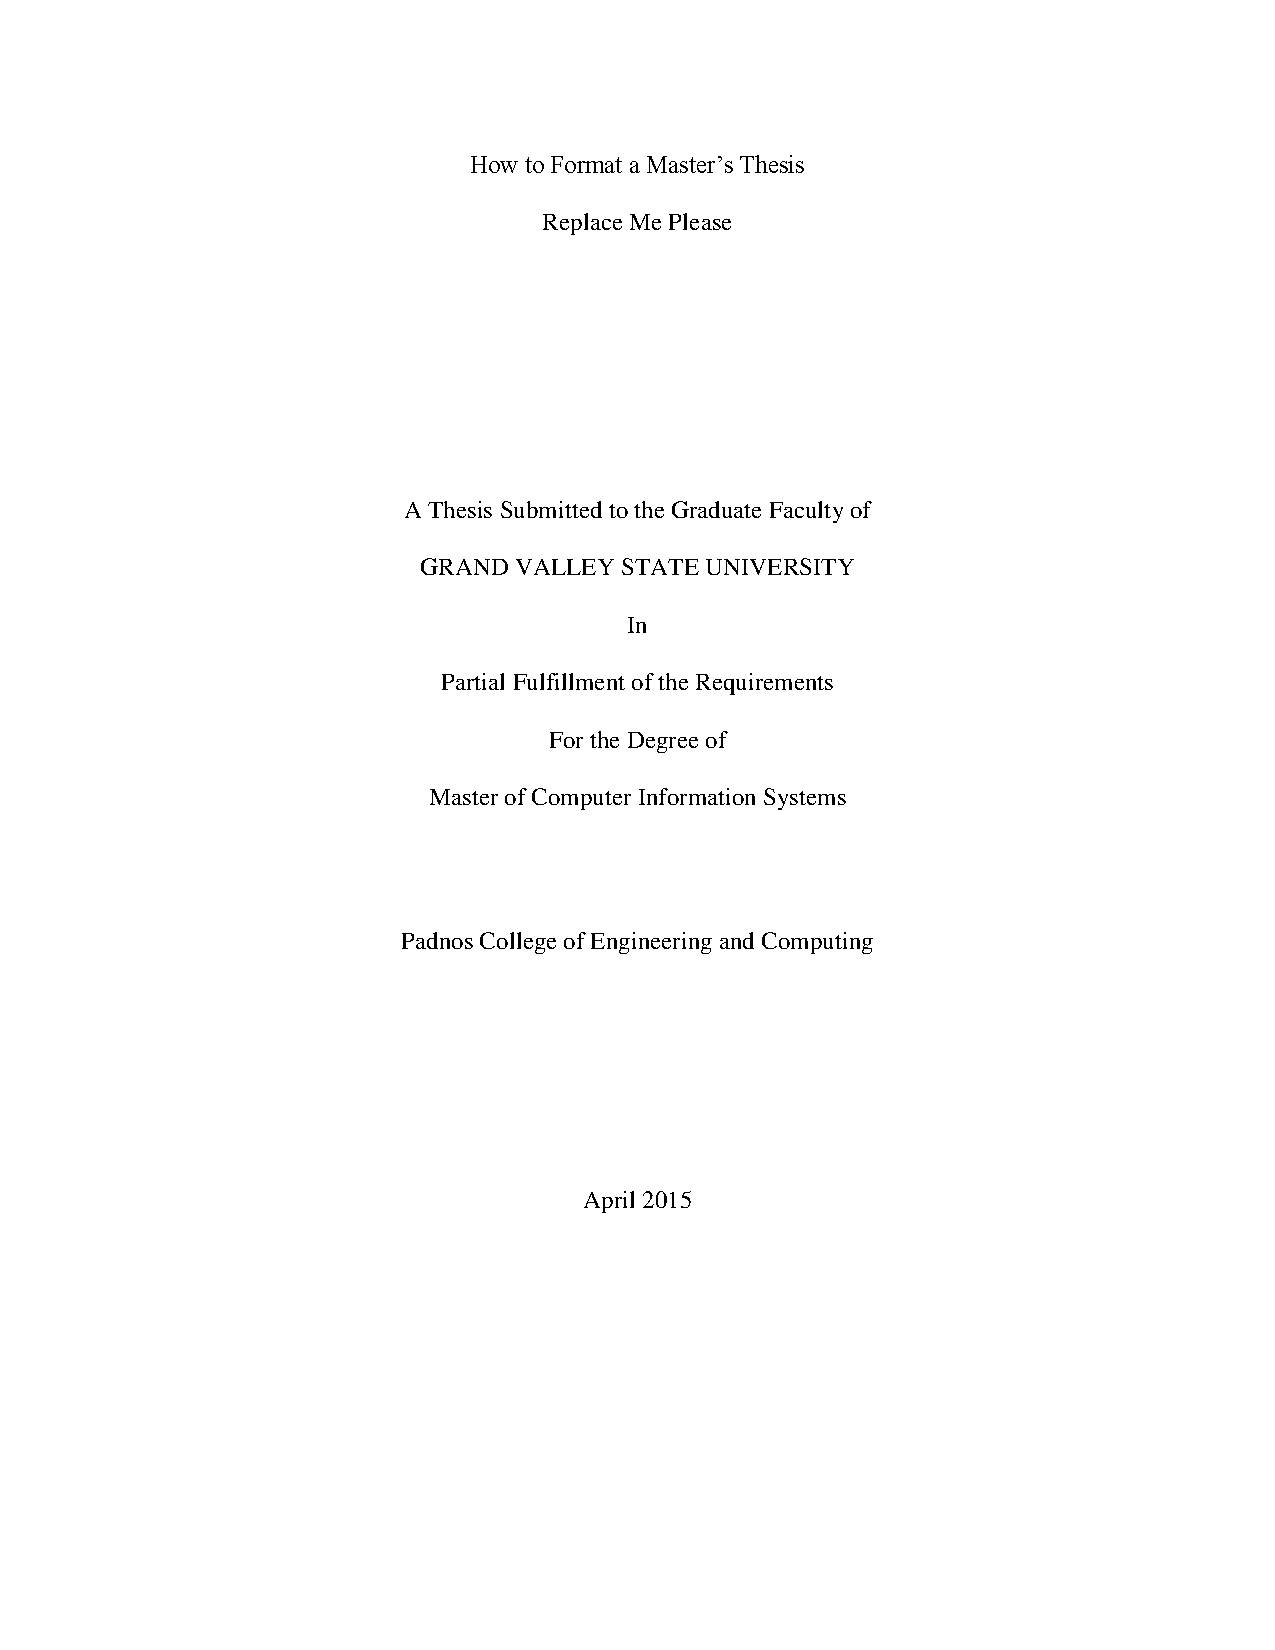
\includepdf{ogs-forms/filled/titlepage.pdf}
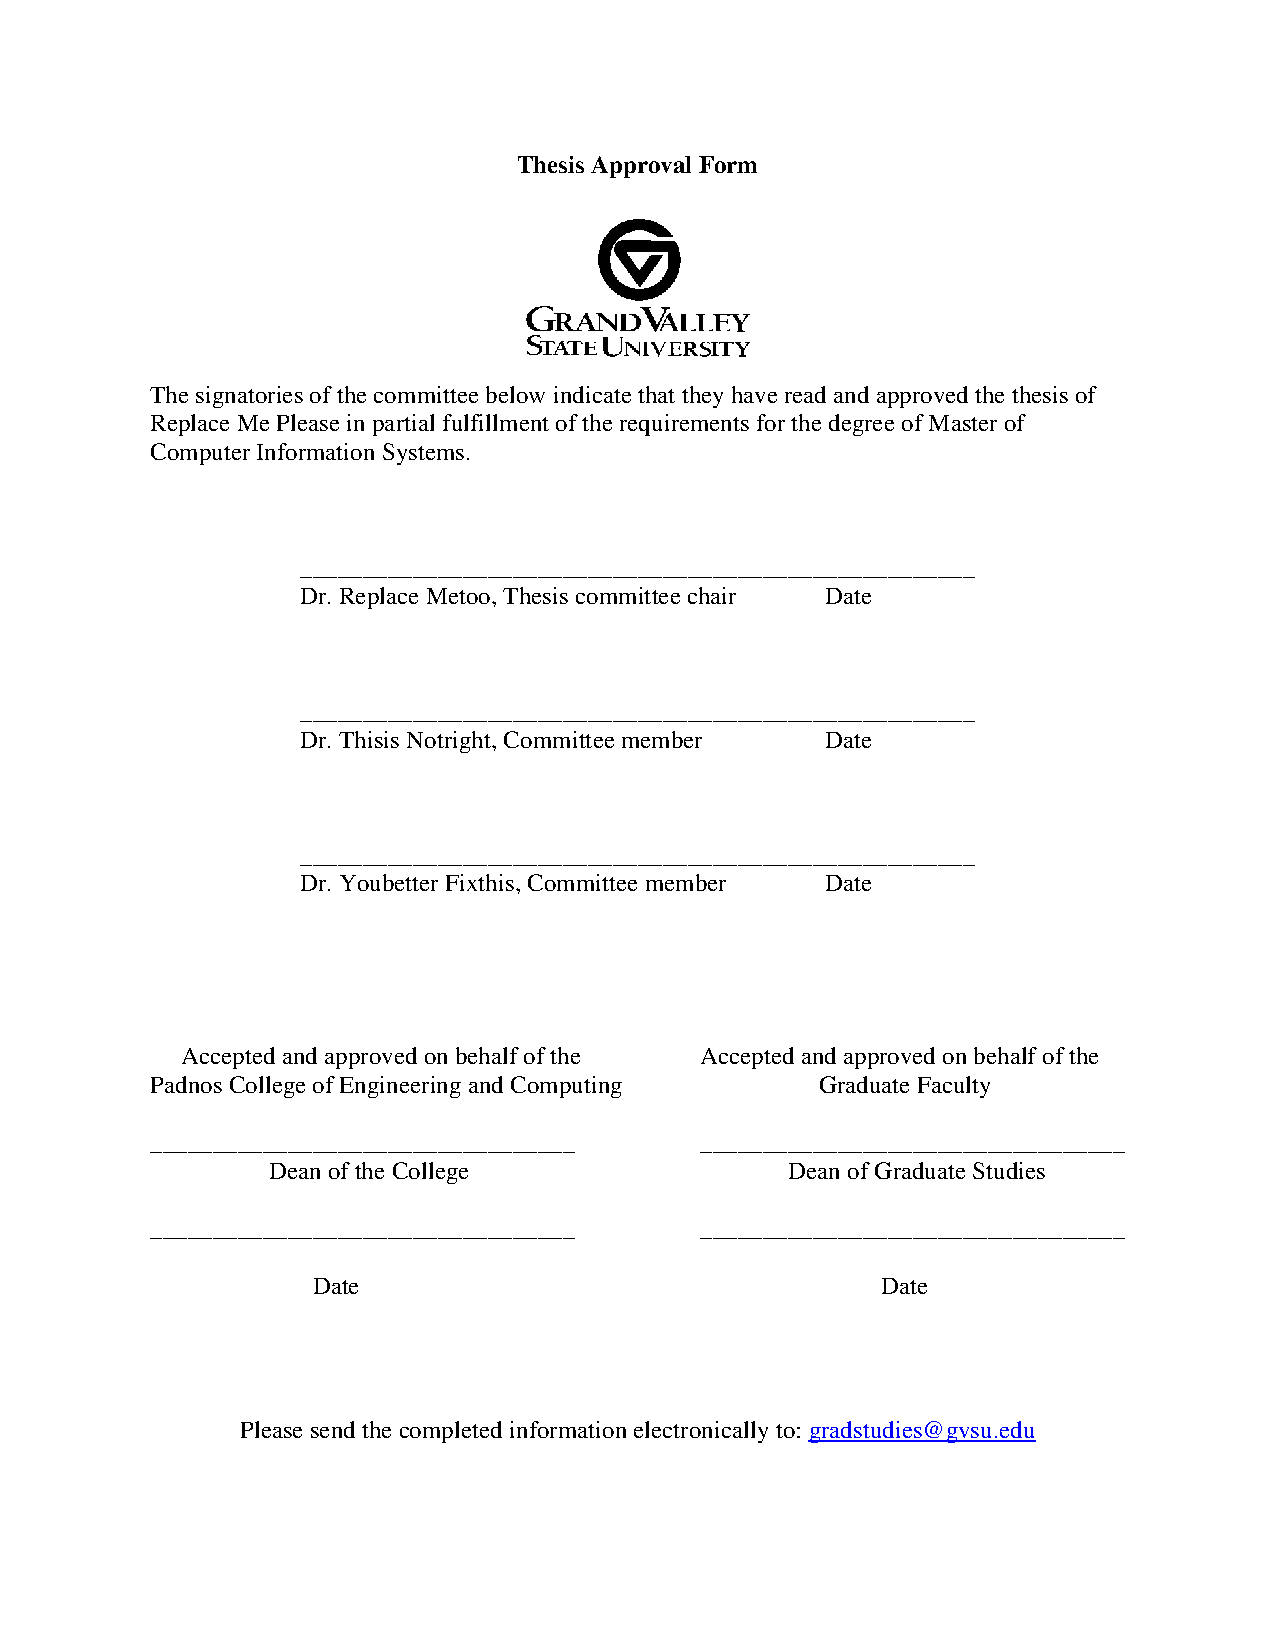
\includepdf[addtotoc={1,addsec,1,Thesis Approval Form,approval-form}]{ogs-forms/filled/approval.pdf}

\doublespacing
\begin{abstract}
  Functional programming presents a relatively unexplored approach to achieving high-performance computing. Typically, the field has been dominated by imperative languages such as C, C++ and Fortran. However, purely functional languages use functions without side effects, a characteristic that can prove useful when parallelizing code. The purpose of this project is to investigate the feasability of an automatic parallelizing compiler for functional programs. Paralisp uses the LLVM compiler infrastructure to transform Lisp-like source code into LLVM bytecode equipped with calls to parallel functions. The LLVM bytecode is then used to generate Intel x86 machine code that executes within multiple threads. Parallelism is clearly a critical part of today's technological environment, but presents difficult challenges to developers. Much as optimizing compilers for high-level languages have supplanted hand-written assembly, automatic parellelizing compilers optimized for specific architectures are poised to eliminate error-prone manual multiprogramming.
\end{abstract}
\newpage

\singlespacing
\tableofcontents
\newpage

\listoffigures
\newpage

\newgeometry{left=1.5in,right=1in,top=1in,bottom=1in}
\pagenumbering{arabic}
\doublespacing
\section{Introduction}

Increased execution speed has traditionally been achieved in hardware through the acquisition of processors posessing a higher clock rate and in software through manual optimization. However, as demand for faster processing continues to grow, alternative methods of achieving speed with computers have become more popular. The most widespread of these is parallel processing. Computer programs typically are run in a sequential order on a single processor. It is a simple and effective approach. However, programs with a single order of executing instructions fail to take advantage of additional processors or entire machines that may be available. Parallel processing occurs when one cohesive program is run over multiple processors simultaneously.

Currently, the two most widespread approaches for parallel processing are message-passing and multithreading. Message-passing involves explicitly sending messages between processes. The most popular instance of message-passing in action is the Message Passing Interface (MPI) \autocite{gabriel04:_open_mpi}. Although MPI programs can achieve significant speedup, writing them involves considerable programmer effort and is tedious at best.

Multithreading involves spawning multiple lines of execution (threads) within one process, sharing memory between each of the threads. Writing multithreaded programs is easier than writing message-passing programs because memory is implicitly shared, but it results in a less clear separation between shared and unshared memory. Although there are many thread implementations, the most popular is POSIX threads (pthreads) \autocite{pthreads}. Open Multiprocessing (OpenMP) is a declarative multithreading interface built upon on compiler directives which attempts to make multithreaded programming easier \autocite{openmp-specs}.

However, development using explicit parallelism is difficult, error-prone, and time-consuming. The resulting programs are also often non-deterministic. Therefore, automation of the process is very advantageous and is often considered the ``holy grail'' of parallel processing. All of the aforementioned solutions assist in the parallel processing problem, but involve manual code modifications ranging from minimal changes to a re-work of the entire program. Of the aforementioned solutions, OpenMP's declarative interface is closest to implicit parallelism. However, OpenMP is at the same time wholly \emph{not} automatic parallelism since it requires specific code modification. In addition, adapting a program to use OpenMP's directives may require some reworking. True automatic parallelization requires no code modification.

Automatic parallelization is not without its difficulties. Its main challenges are task extraction and data hazard handling. This is where functional programming languages can prove beneficial.

Functional languages are a special breed of language that treat programming as the evaluation of mathematical functions. By doing so, they avoid carrying state through the computation of function results. This property assists greatly in avoiding data hazards that occur in typical procedural programs. This property can also prove useful when tackling the problem of task extraction, although that topic is not addressed in this project.

In recent years, the amount and variety of programming languages has exploded. New paradigms have even been introduced. The introduction of high-level scripting languages such as Python, Ruby, and Lua has made programming easier than ever.

However, these advancements have been slow to permeate the area of parallel processing and the field of high-performance computing in general. The reference implementations of Python and Ruby (CPython and CRuby) both use a \emph{global interpreter lock}, a mechanism which prevents an interpreter from running multiple programs simultaneously within the same process. Global interpreter locks are typically used to speed up the execution of single-threaded programs and for ease of implementation. However, this effectively prevents multithreading for performance gains and is a major hindrance to achieving full parallelism.

In addition, while the number of interpreted languages is steadily increasing, new traditional compiled languages are relatively rare. There are many reasons behind this trend. Developing production-quality compiled languages and compilers requires far more detailed work and is much more time-consuming than producing interpreted languages. Furthermore, compilers for older languages have had many years of tweaking and optimization. The result of this is that new high-level compiled languages with high performance and good support for parallelism are few and far between.

Therefore, parallel processing has traditionally been implemented in low-level existing compiled languages such as C, C++, and Fortran. This is due to the perceived need to be ``close to metal'' in order to squeeze every last bit of performance out of the code. This typically involves manually tweaking algorithms to get the most efficient parallelism possible, yielding the greatest speedup.

Automatic parallelizing compilers address the parallelism problem in a completely different way. Instead of providing interfaces for parallelism at the language or library level, these compilers implement parallelism within the compiler itself. This shifts the burden of implementing parallelism from the language developer to the compiler developer. For the language developer, this enables effortless parallelism at the cost of losing control over the way the parallelism is implemented. However, this makes automatic paralellizing compilers much more difficult to write than traditional compilers.

Paralisp is an implementation of an automatic parallelizing compiler for a select subset of a functional language. Focus is placed on program correctness and potential speedup. Results and execution time are benchmarked against a single-threaded program and a hand-optimized program using explicit parallelism.

\section{Background}

\subsection{Compiler Design}

Typical compilers have multiple stages which usually include lexical analysis, semantic analysis, code generation, and an optional optimization phase.Additional optimization can optionally take place within or between any of these states as well. Lexical and semantic analysis are together referred to as the compiler \textit{frontend}. The frontend primarily deals with the syntax and appearance of the language. Code generation and optimization make up the compiler \textit{backend}. The backend takes the output of the frontend and transforms it into code that can be executed on a specific architecture.

Together, these stages transform a program's textual source code to machine code or intermediate bytecode. A program compiled to machine code can be run directly on the processor. A program compiled to bytecode is translated to machine code at runtime by a virtual machine such as the Java Virtual Machine or Common Language Runtime (the .NET virtual machine).

Lexical analysis, or scanning, is the process of separating input text into meaningful tokens. In a Lisp-like functional language, this involves detecting tokens such as parentheses, the function name, and function inputs. Consider the following Lisp-like expression:

\scheme|(print (+ 4 7))|

In this expression, eight tokens would be produced: \verb|(|, \verb|print|, \verb|(|, \verb|+|, \verb|4|, \verb|7|, \verb|)| and \verb|)|. These tokens constitute each meaningful piece of the expression. Although the meaningful parts are distinguished from one another, their meaning is not yet assigned. Assignment of meaning occurs during the next step, parsing.

\begin{figure}
  \centering
  \scheme|(+ (- 10 2) (* 3 4))|
  \caption{Lisp expression to parse}\label{fig:lisp-parsing}
\end{figure}

Semantic analysis, or parsing, is the process of assigning meaning to tokens. The end result of parsing is the construction of an \textit{abstract syntax tree}, a data structure that organizes those meaningful parts of the code in a hierarchical manner. An example of parsing a Lisp program that uses only arithmetic expressions is shown in \Fref{fig:lisp-parsing}.

The third step of compilation is code generation. Code generation involves transformation of the abstract syntax tree into a form executable by a runtime, the operating system, or the machine itself. This is often the most challenging step because in-depth knowledge of each target platform is usually necessary to output code that will run correctly. As such, code generation is a notoriously difficult stage of building a compiler. However, this challenge can be partially mitigated by good tools.

\subsection{The Functional Advantage}

Historically, functional languages have typically been relegated to academic and research projects. Although their origins were far in the past (Lisp was introduced in 1958), they have never been popular in mainstream programming apart from artificial intelligence and Emacs. They have rarely been used in the field of high-performance computing, where low-level languages such as C, C++, and Fortran dominate the field. However, functional languages have an important property that assists greatly in the implementation of automated parallelism.

The basis of most functional languages is the \emph{pure function}. A pure function maps arguments to a value and has no external effects other than the value returned to the function's invoker. In short, a pure function is stateless and side-effect free \autocite{10.1109/MCSE.2012.69}.

Both absence of state and absence of side effects are important when considering pure functions. A stateless function's output is not affected by anything other than its inputs. The state of memory outside the function cannot affect its return value. A side-effect free function cannot affect anything other than its output. A side-effect free function may not modify any value besides local variables and its return value. A function must be stateless and without side effects to be considered a pure function.

Pure functions are very beneficial when dealing with parallelism. Without state or side effects, any given function cannot write to shared program memory. This means that there is no chance of any function overwriting another's value, and eliminates the need for data synchronization mechanisms such as mutexes and semaphores. As a result, the entire program structure can be decomposed into a call graph tree of independent, stateless functions, which can then be run in parallel without risk of data hazards.

However, most functional languages are not pure functional languages. For example, Common Lisp also includes aspects of procedural and object-oriented programming. Paralisp considers only pure functions executed in parallel.

Although pure functional languages eliminate data hazards, they are no silver bullet to solving the problem of automatic parallelization. There are still many issues that remain, including task extraction, task granularity selection, and task scheduling \autocites{Girkar:1995:ETP:210184.210189}{improving-task-scheduling}.

\subsubsection{Parallel Task Extraction and Granularity}

Task extraction refers to the division of code into separate chunks to be executed on individual processors. So-called ``embarrassingly parallel'' tasks can be parallelized with a minimum amount of coordination between executing processes. Task granularity refers to the size of each of these tasks. Most parallel tasks, however, require a moderate to high amount of communication and synchronization. A medium must be found between task granularity and cost of communication. Smaller tasks mean a higher degree of parallelism at the cost of more communication overhead. Larger tasks mean that more code can be executed in sequence on each processor, but with a lesser degree of parallelism.

Two types of task parallelism exist: structured and unstructured parallelism \autocite{Girkar:1995:ETP:210184.210189}. Structured parallelism is primarily applied to loops. This is the approach that OpenMP takes when parallelizing code. Individual loop executions are typically designed to execute on data independently, which allows creation of a list schedule that executes on multiple processors. Structured parallelism is simple yet effective, which is why it has come into mainstream use. However, it usually requires manual annotations to be placed on each loop to run in parallel.

Unstructured or functional parallelism allows for greater flexibility than structured parallelism. In addition, unstructured parallelism can be determined without need of manual code annotations. However, this comes at a cost: unstructured tasks are more difficult to extract. Added to this challenge is the process of automatically determining the granularity of the extracted task. Unstructured task extraction must also take into account control and data dependencies. Control dependencies refer to branches of code (e.g., conditionals, loops, or function calls) which may execute conditionally and whose actions are difficult to predict. Data dependencies refer to results produced as output of a task that must be given as input to another task.

Paralisp is a proof-of-concept compiler focused only on automated structured parallelism. It does not require any change of code such as annotations or calls into parallel libraries. The operation that is parallelized is the common functional \verb|map| operation.

\section{Implementation}

\subsection{Flex}

In Paralisp, lexical analysis is performed with a scanner generated by Flex, the fast lexical analyzer \autocite{flex}. Flex is an implementation of the standard UNIX tool Lex\@. Flex and other Lex implementations are given as input a set of rules composed of regular expressions and actions to take when they are matched. From these rules, Flex is able to generate code for a scanner. This code is then integrated with the rest of the compiler into an executable. Although the traditional interface is output in the C programming language, Flex also offers the option to output an interface in the C++ programming language which places the scanner code in a containing class. Other than containment, the C++ output offers little additional value.

\subsection{Bison}

Paralisp uses a parser generated by GNU Bison \autocite{bison}, the GNU implementation of the standard UNIX tool Yacc. In the same vein as Flex, Bison generates code for a parser from a set of rules given in its input file. Although Flex and Bison are similar in this way, the task that Bison performs is much more involved than the task that Flex performs, and Bison is the more important tool. However, Flex and Bison were designed to be used together and therefore make good choices for construction of a compiler frontend. Like Flex, the parser generated by Bison can either be output in C or C++, with an additional experimental Java output. Unlike Flex, however, Bison's C++ output offers significant advantages.

The Bison C interface requires a homogenous data structure in which to place parsed nodes. Traditionally, this is a C union. However, unions are notorious for their loss of type information with respect to their contents. Access to fields of a union is usually predicated on assumption, which also makes it hard for the compiler to warn about possible issues. Although field access issues do not typically arise with use of unions in Bison, the possibility is always important to keep in mind. Furthermore, unions in C++03 can only store so-called plain-old-data (POD) types, meaning that the oft-used \verb|std::string| is excluded. The string type \verb|std::string| can only be used by storing a pointer to it, which is an inconvenience. It also unnecessarily complicates the memory managment of parsed nodes.

However, when selecting C++ as the output language, Bison offers a choice between the traditional unions and a C++ variant type. The Bison C++ variant type offers the advantage of being able to store non-POD data, which greatly simplifies memory management. It also has the advantage of being more strict with its typing, meaning that incorrect assignments are likely to be detected sooner.

Unfortunately, the Bison C++ variants are not recursive, i.e., Bison does not have support for recursive variants. This is because Bison needs concrete definitions of each of the types that will be stored inside of the variant to determine the maximum size of the variant. This is not a problem for simple Lisp terminal nodes such as identifiers or integers, which cannot contain any child nodes. However, the Lisp list data struture is designed to store other lists, meaning a recursive definition is necessary.

Fortunately, Bison variants \emph{can} store other types that do support recursive definition, such as Boost's variant type. Boost.Variant is described in greater detail in \Fref{sec:boost}.

\subsection{LLVM}

Paralisp uses the LLVM compiler infrastructure for the code generation stage. LLVM is a complex toolchain, but is very full-featured and one of the best options available for this task. Chris Lattner, the primary author of the LLVM project, describes it as a language independent optimizer and code generator whose goal is to build a set of modular compiler components \autocite{2011-02-FOSDEM-LLVMAndClang}. LLVM allows for code generation using a constructive programmatic interface written in C++.

Instead of directly using, for example, the Intel x86 assembly language, LLVM uses a special high-level assembly language called the LLVM Intermediate Representation (LLVM IR). The LLVM IR comes in three different forms: a textual assembly language form that is readable by humans, an in-memory representation as used by a compiler, and a binary bitcode representation that can be stored on disk. Although each form is distinct, they represent the same operations and data and can usually be used interchangably. Additionaly, the LLVM IR uses static single assignment form (SSA), which guarantees that each created variable is assigned only once. Among other uses, SSA's foremost benefit is facility of compiler optimizations. SSA also fits extremely well with the functional paradigm which eschews mutable data.

The code for Paralisp is based in large part on \citeauthor{toy-compiler}'s excellent tutorial \citetitle{toy-compiler} \autocite{toy-compiler}. The tutorial takes the reader through building a simple compiler for a C-like language using the aforementioned tools. However, the code suffers from a number of deficiencies: memory leaks, deprecated LLVM calls, and a somewhat inflexible design. Nevertheless, this code served as an excellent starting point for building a compiler for a Lisp-like language using LLVM\@. Paralisp's codebase was originally based on this tutorial, although it now bears little resemblance to the original code.

Another tutorial which was referenced heavily in the building of Paralisp is \citeauthor{llvm-kaleidescope}'s excellent LLVM tutorial, \citetitle{llvm-kaleidescope} \autocite{llvm-kaleidescope}. Because this tutorial is part of the official LLVM documentation, it focuses more on useful and exotic features of LLVM, choosing to implement its own lexer and parser with admittedly less-than-ideal global state. However, this tutorial also instructs the reader in building support for conditionals and enabling optimizations, the first of which is very important to Paralisp's implementation.

Unfortunately, both tutorials only take the code generation as far as LLVM intermediate language. Although simple LLVM IR can be interpreted or transformed into a state in which it can be run, it cannot be run on its own. Furthermore, more complex LLVM IR which has external dependencies is more difficult to manage and requires special steps to be run on its own. However, users of a compiler expect the compiler to produce an executable which can be run without modification. They do not expect to have to run additional steps to get a working program. Paralisp satisfies this expectation by running the extra steps automatically as part of the normal compilation process.

Part of the LLVM toolchain that has proven extremely useful is its ability to seamlessly convert between different representations of the same code. LLVM IR serves as a junction between several different formats, including C, C++, and our own Lisp source code. The most useful feature is part of \texttt{llc}, the LLVM static compiler. By using the \texttt{llc} command line option \texttt{-march=cpp}, LLVM will take the given intermediate representation and output the necessary LLVM C++ API code to build that code in memory. This can be combined effectively with Clang, a C family frontend for LLVM \autocite{clang}. This combination can be used to view the LLVM C++ API code for the following small C snippet illustrated in \Fref{fig:llvm-api-for-c}. In addition, the \citetitle{llvm-demo} (now offline) and \citetitle{ellcc-demo} pages provide this feature via an easy-to-use web interface \autocites{llvm-demo}{ellcc-demo}.

In practice, the API code output by these tools is never used directly. Most often it is converted to use nicer interfaces like LLVM's \texttt{IRBuilder<>} or simply made more readable. However, this type of code proves invaluable when trying to implement more exotic LLVM features, such as code that passes and calls through function pointers or deals with arrays. Although these type of operations are not documented in great detail in LLVM's official documentation, these tools provide a simpler mechanism: If you can write it in C or C++, then LLVM will show you how to write it in its own API code. This is a truly amazing feature which has torn down many roadblocks during the construction of the compiler.

Finally, the most reliable and time-honored way of getting help is by reading sources. This applies even more than usual when using LLVM\@. Fortunately, Clang is an existing production-quality compiler for C, C++, and Objective-C which showcases the best uses of LLVM\@. Much of the compilation functions used in Paralisp were adapted from Clang or \texttt{llc}, the LLVM static compiler.

\begin{figure}
  \inputminted[tabsize=4,frame=single,label=funcptr.c]{c}{code/funcptr.c}
  \inputminted[frame=single,label=Command line]{bash}{code/clang-llc-funcptr.bash}
  \caption{LLVM C++ API code for C code}\label{fig:llvm-api-for-c}
\end{figure}

\subsection{Language of Implementation}

The primary motivating factor in deciding the language of implementation was the use of LLVM\@. LLVM is implemented in C++, so it is unsurprising that its native interface is also in C++. Although LLVM provides interfaces for C, Python, and others, these interfaces do not expose the full functionality of LLVM\@. When working with libraries, it is important to remember that libraries \emph{always} work best with their native interfaces. In fact, it is typical for non-native interfaces to expose only partial functionality, lag behind in terms of reliability and features, and to be eliminated entirely when they become too burdensome to maintain. It is for this reason that C++ was chosen as the language of implementation.

\subsection{C++11 vs. C++03}

After deciding on C++ as the language of implementation, the decision of which C++ version to use came into focus. The two major standards of C++ currently in use are C++11 and C++03. According to \citeauthor{bs-faq}, C++03 is basically C++98 with bug fixes and therefore can be used interchangably by programmers \autocite{bs-faq}. C++11, formerly known as C++0x, is the newest revision to the C++ standard. While C++03 is not outdated, C++11 provides a number of useful features that ease development and provides functionality previously only found in external libraries.

A C++11 development environment requires two distinct parts: language support from the compiler and library support from the C++ standard library implementation. Clang with libc++ has a full implementation of C++11 as well as C++14, and GCC with libstdc++ has a mostly complete implementation of C++11. Microsoft's Visual C++ compiler is lagging behind slightly, but is adding more C++11 features as time goes on.

C++11 was the desired language of implementation for Paralisp. However, it is not the compilers nor the libraries that make C++11 difficult to use. It is primarily the operating system vendors and the nature of the distribution of a C++ compiler and standard library.

A shared C++ standard library is a standard part of any modern operating system. Likewise, a C++ compiler is a standard part of any development environment. Unfortunately, most tools surrounding a C++ environment expect \emph{only one} of each of these components to be installed on a system at a given time. Since these two pieces are so crucial to a functioning operating system, most vendors distribute these in a structured, pre-ordained way which is not designed to give the user customization and control over the environment.

All these factors conspire to make a successful C++11 environment very difficult to realize on systems not specifically designed for it. Numerous issues including non-standard paths, incompatible interfaces, incompatible versions, and incorrect library linkage have been encountered. Furthermore, successful setups differ even between versions of the same operating system.

When the project started, the conclusion was that C++11 was not the best choice for compiling and distributing portable programs, and the decision was made to use C++03. The hopeful note to this debate is that the C++11 situation is rapidly improving.

\subsection{Boost}
\label{sec:boost}

The Boost C++ libraries are used pervasively throughout this project. For C++ developers, the Boost libraries need no introduction. For others, the Boost C++ libraries are a set of high-quality portable libraries that make development in C++ much more enjoyable. Many of the Boost libraries go into C++ Technical Reports (TRs) and eventually become part of the C++ standard library. In fact, Boost can serve as a sort of ``C++11 for C++03'' due to the amount of Boost libraries that have entered the C++11 standard library. However, Boost also contains libraries that will never make it into the standard library. In this way, Boost can be viewed as a batteries-included catch-all library in that it contains many useful wheels which would otherwise have to be reinvented.

Paralisp makes heavy use of Boost. Boost Bind and Function are used to delay function calls by storing the function and its arguments in a cohesive structure. Boost Filesystem, Thread, and Timer are useful to provide unified interfaces to platform-specific features, while Boost Predef allows safe access to platform-specific APIs with operating system detection macros. Boost Unordered provides hash-based maps and sets which make up for C++03's lack of these absolutely necessary amortized constant-time data structures. Boost Algorithm, Foreach, and Lexical Cast are used as general utilities.

Boost Program Options provides a generic but full-featured command-line option and argument parser interface. Like a typical compiler, Paralisp takes many command-line flags which serve to customize the output. Although parsing command-line options may seem like a relatively simple and mundane task, it is in fact a complex task which requires considerable care and practice to get right. While Program Options does not cover every possible case and possesses some quirky behavior when it comes to positional arguments, it is overall a high-quality library which greatly simplifies this error-prone task.

Boost.Variant is the most significant Boost library used in Paralisp. Boost.Variant is an implementation of a discriminated or tagged union, a data structure which is capable of storing a fixed set of different types. Boost.Variant also provides other beneficial features, such as an implementation of dynamic dispatch. The Boost.Variant design is described further by \citeauthor{boost-variant} in \citetitle{boost-variant}, and more of its benefits are described in \Fref{sec:dyn-disp}.

\subsection{Parallelism}

\begin{figure}
  \begin{subfigure}[b]{0.5\textwidth}
    \centering
    \inputminted{scheme}{code/map-is-positive.scm}
    \caption{Code}
  \end{subfigure}
  \begin{subfigure}[b]{0.5\textwidth}
    \centering
    \verb|List: 0 1 0 0 0 1 1|
    \caption{Output}
  \end{subfigure}
  \caption{Using map}\label{fig:map}
\end{figure}

Parallel execution is implemented for Paralisp's \verb|map| function. \verb|map| is a function found in most functional programming languages in addition to many languages that include features of a functional paradigm. Its operation is relatively simple. It accepts two arguments: a sequence and a transformation function. The function is then applied to each element of the sequence to produce a new list. In our case, the transformation function must be a pure function as defined earlier.

The \verb|map| operation is a great candidate for parallelism because it does not specify how or when the transformation function is run on each of the elements. Furthermore, each transformation can be executed concurrently because of lack of dependency between them.

The concurrent execution of \verb|map| is implemented within Paralisp's standard library. Boost Thread is used for portable multithreading. Independent \verb|map| iterations are executed simultaneously by spawning a number of threads corresponding to the number of processors as reported by the operating system.

The standard library contains two functions, \verb|map-sequential| and \verb|map-parallel|. By default, a call to \verb|map| is instructed to call \verb|map-sequential| internally. Parallel map execution is activated by passing either the \verb|--parallel| or \verb|-P| option to Paralisp, which causes \verb|map| calls to internally call \verb|map-parallel|. An example program which utilizes \verb|map| is shown in \Fref{fig:map}.

\subsection{Dynamic Dispatch}
\label{sec:dyn-disp}

\begin{figure}
  \centering
  \verbatiminput{code/dyn-disp/out.txt}
  \caption{Output generated by all dynamic dispatch implementations}\label{fig:dyn-disp-out}
\end{figure}

\begin{figure}
  \centering
  \inputminted[fontsize=\scriptsize,tabsize=4]{cpp}{code/dyn-disp/cxx-rtti-virtual.cpp}
  \caption{Dynamic dispatch with C++ RTTI and virtual functions}\label{fig:dyn-disp-cxx}
\end{figure}

\begin{figure}
  \centering
  \inputminted[fontsize=\tiny,tabsize=4]{cpp}{code/dyn-disp/llvm-rtti-virtual.cpp}
  \caption{Dynamic dispatch with LLVM RTTI and virtual functions}\label{fig:dyn-disp-llvm}
\end{figure}

\begin{figure}
  \centering
  \inputminted[fontsize=\scriptsize,tabsize=4]{cpp}{code/dyn-disp/boost-variant-visitor.cpp}
  \caption{Dynamic dispatch with Boost.Variant and the visitor pattern}\label{fig:dyn-disp-boost}
\end{figure}

The output of Paralisp's parsing stage is an abstract syntax tree, which is a tree of specific types of nodes which have been given meaning. For example, two different types of nodes that are seen in the Paralisp language are identifiers and integers. Each of these types of nodes is distinct and requires distinct actions to be taken in order to generate the proper code.

To generate code, a pre-order traversal is applied to the tree. Traversing the tree consists of application of an algorithm to a heterogenous set of nodes. This is implemented by creating a virtual function as part of each node class. However, restrictions of Bison, C++ data structures, and our own data structures require that data being stored in these structures be homogeneous. This means that the classes stored must have a consistent interface.

By default, C++ uses static dispatch, which means that it selects the method to run at compile-time. A base \verb|Node| type cannot be stored in the data structures else the \verb|Node| implementation of the code generation method would always be selected at runtime.

The solution to this problem is dynamic dispatch: the method to run is chosen at runtime. Two different implementations of dynamic dispatch are explored: nodes accessed through pointers with virtual function calls, and nodes accessed through variants with the visitor pattern.

Within these two implementations, three possible methods of implementation are discussed: built-in C++ run-time type interaction (RTTI) with virtual function calls, LLVM RTTI with virtual function calls, and Boost.Variant with use of the visitor pattern. Each implementation produces the same output, which is shown in \Fref{fig:dyn-disp-out}.

A sample C++ implementation is shown in \Fref{fig:dyn-disp-cxx}. It is rather standard, using the built-in C++ RTTI for the \verb|dynamic_cast<>| operation and virtual functions for dynamic dispatch. It is relatively straightforward and works well for simple tasks.

LLVM possesses its own form of RTTI instead of the built-in C++ RTTI\@. It is used within LLVM, but can also be used for user class hierarchies. According to \citeauthor{so-llvm-rtti}, it was developed primarily for reasons of performance \autocite{so-llvm-rtti}. C++ RTTI requires a vtable, meaning that a class must have at least one virtual function. This and other areas of built-in C++ RTTI can waste space. In addition, the LLVM developers were unhappy with the performance of run-time checks done by C++ RTTI\@. Although LLVM RTTI allows for more efficient checks and more flexibility, it requires quite a bit more work from the developer. A sample implementation using LLVM RTTI is shown in \Fref{fig:dyn-disp-llvm}.

While standard C++ and LLVM implement more or less the same interface, use of Boost.Variant provides a drastically different interface by separating the algorithms from the data structures on which they operate. Although it adds a small amount of boilerplate code, it is not nearly as much as the LLVM implementation.

Boost.Variant utilizes the visitor pattern in order to execute operations on each node. Virtual functions are preferrable when there are a fixed set of operations and a variable number of types, while the visitor pattern excels at operating on a fixed set of types with multiple operations. In this case, our application has more diverse operations than types, making the visitor pattern a good choice. In addition, Boost.Variant makes extending both the types and operations simpler by allowing templated operations.

In the end, the visitor pattern's most notable advantage is one of scope. By separating the algorithms from the data structures on which they operate, data structures which have no knowledge of those algorithms can be used. This allows infinte augmentation of the algorithms with more operations while at the same time leaving the data structures untouched.

\subsection{Standard Library}

Many of Paralisp's simple operators are implemented by outputting pure LLVM bytecode. This approach works well for arithmetic operators, conditionals, user-defined functions, and function calls. In general, this approach works best for simple blocks of code or blocks of code which are built from the ground up. However, this approach proves difficult when the aim is to execute an existing function of substantial size. To get this to work, one would have to craft LLVM C++ API code to make the proper calls to other functions. This becomes tiresome rather quickly.

This is because the LLVM C++ API is designed to be called to \emph{generate} LLVM bytecode from another representation (e.g., Scheme source) rather than express existing functions. This is where LLVM's C and C++ interoperability becomes invaluable.

LLVM uses C calling conventions, which means that LLVM bytecode can call out to functions within any C library. Realizing the availability and importance of this feature was paramount in making Paralisp work as it should. LLVM can also call functions written in C++. However, since C++ uses name mangling, it is necessary to surround the C++ function with an \verb|extern "C" { ... }| declaration to disable it. The code within each function can be written in either C or C++; it makes no difference to LLVM.

The code for the standard library is compiled into a static library which is used in the linking step.

\subsection{Creation of an Executable}

Paralisp begins by reading the user's source code and processing it by scanning, parsing, and generating until the code is in an in-memory format held by an LLVM \verb|Module|. At this point, LLVM has enough information to create executable code.

However, the farthest point to which LLVM can go is to a file containing the native assembly language of the platform. This native assembly can be then fed to the native assembler (usually called \texttt{as}) to produce an object file (*.o). The LLVM tool \texttt{llc} has an experimental mode which compiles to binary object files that may be investigated at a later time.

Note that no sort of code or file that can be directly executed on the system has yet been reached. The final step which remains is to link everything together to create the final executable. This includes the object file produced by the user code and all libraries upon which that object file depends. These include the Paralisp standard library, the Boost and GraphicsMagick libraries needed for the Paralisp standard library, and the C++ standard library needed for the Paralisp standard library, Boost, and GraphicsMagick. GraphicsMagick is used here for the image input and output used in the test program. These libraries can be static or shared, although the Paralisp standard library is currently always compiled as a static library. This step is performed using \texttt{ld}, the GNU linker. LLVM also has a new project called \texttt{lld} which is intended to replace the GNU linker, but it is currently not ready for production usage.

After linkage, the result is an executable file capable of being run natively on the system.

\section{Results}

Benchmarking a compiler's output executable performance requires a program to be written as input to the compiler. For this program, the topic of image processing was selected. The threshold operation, which segments a grayscale image into a bi-level image which contains only black and white, was selected as a compromise between interesting results and ease of implementation.

\begin{figure}[p]
  \centering
  \begin{subfigure}{0.8\textwidth}
    \includegraphics[width=\textwidth]{images/carina-in-color}
    
\includegraphics[width=\textwidth]{images/carina-in-grayscale}
    \caption{Input}\label{fig:carina-in}
  \end{subfigure}
  \begin{subfigure}{0.8\textwidth}
    
\includegraphics[width=\textwidth]{images/carina-out}
    \caption{Output}\label{fig:carina-out}
  \end{subfigure}
  \caption{Carina Nebula --- Hubble Space Telescope}\label{fig:carina}
\end{figure}

The benchmark starts with a grayscale image of the Carina Nebula taken by the Hubble Space Telescope. This image is also shown in color for reference. Although our program can operate on color images, they are converted to grayscale before beginning the operation. Both the color and grayscale images are pictured in \Fref{fig:carina-in}.

This image was chosen because of the interesting pattern and high resolution. The original image, which was scaled down for publication of this paper, has a resolution of 29566 by 14321 pixels. This was thought to require enough computation to challenge the bounds of the program.

Other than to demonstrate and benchmark the Paralisp compiler, the goal of this program is to distinguish stars in the Carina Nebula by using the thresholding operation to remove the ``cloud'' which surrounds them. Since the color of the cloud is not as bright as the stars, a high color value with which to discriminate them has been chosen.

\begin{figure}
  \centering
  \inputminted{scheme}{code/image-threshold.scm}
  \caption{Image threshold program}\label{fig:image-threshold-program}
\end{figure}

The program shown in \Fref{fig:image-threshold-program} was compiled with Paralisp and executed on the grayscale Carina Nebula image. The standard library procedure \verb|list-from-image| reads an image, \texttt{in.jpg}, from the current directory and forms its pixels into a Paralisp array. The pixels have a quantum depth of 8, meaning their value ranges from 0 to 255, 0 being black and 255 being white. Each of the pixels is passed to the \verb|threshold| function through the \verb|map| operation. The \verb|map| function returns an array with each element being either 0 or 255. The \verb|image-from-list| function re-forms the list into an image, \texttt{out.jpg}, in the current directory. The dimensions of the image are required because the list received by \verb|image-from-list| is one-dimensional and contains no image dimension information.

The resulting image is shown in \Fref{fig:carina-out}. Most of the cloud has been removed, although remnants of it remain in the center of the left half. The actual image which is produced as output is far more detailed than can be shown here, and shows many stars beneath the cloud.

\begin{figure}
  \centering
  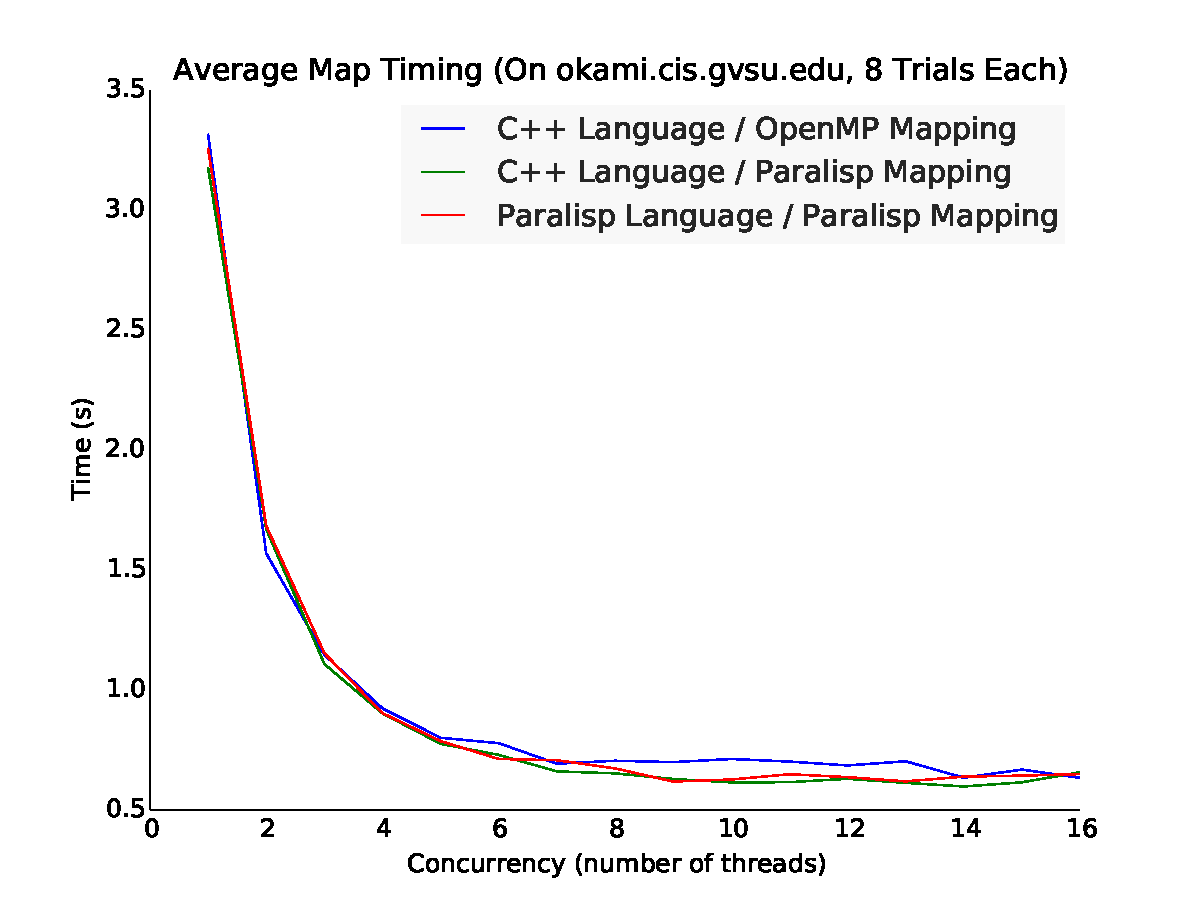
\includegraphics[width=\textwidth]{images/timing-okami}
  \caption{Average map timing on Okami}\label{fig:timing-okami}
\end{figure}

The compiled program was executed on Okami, a 16-processor system located in the DEN, a high-performance computing lab in GVSU's Mackinac Hall. In addition to running Paralisp, two more implementations were also run: a C++ program which uses the Paralisp standard library for mapping and a C++ program which used OpenMP for mapping. The timing and performance results are illustrated in \Fref{fig:timing-okami}.

The results are in general very promising: the two C++ benchmark programs seem to have no advantage over Paralisp. We postulate two reasons for this behavior: Paralisp code is compiled down to machine code, and the operation is relatively simple, giving the C++ compiler little room for optimization. These attributes give the Paralisp and C++ executables relatively equal footing. The OpenMP benchmark shows that the approaches taken by Paralisp and OpenMP in mapping work to each of the threads result in similar performance.

The speedup of each implementation is close to linear until about 7 threads. This is most likely due to the simplicity of the algorithm; at this point, the overhead of creating more threads overwhelms the benefit of parallel processing. In the future, more complex algorithms may be implemented and run with Paralisp. However, more complex operations require Paralisp to support more exotic features, which in turn necessitates additional work on the compiler. In short, the operations necessary for constructing the algorithm must be themselves constructed before the algorithm is written.

\section{Conclusion}

Most existing parallelizing compilers achieve speedup by requirement of manual intervention and use of low-level languages. Paralisp is a real compiler which produces parallelized machine code from a high-level language. Paralisp is able to achieve a significant speedup by exploiting the advantages of functional languages using automatic structured parallelism. Although the language is small and simple, it is a successful proof of concept that automatic parallelism works. Minimal intervention is required to produce parallelized code whose execution time is competitive with hand-crafted parallel code.

\section{Future Work}

In the future, we would like to implement more of the Scheme language so that more complex algorithms can be written. These algorithms can then be benchmarked in a way similar to the threshold algorithm. As mentioned earlier, we would also like to attempt to rewrite the compiler in C++11 when we feel that it is ready.

Writing this compiler has given us an appreciatiation of the general difficulty of language design and compiler construction. There are many paths which arrive at the same result. In selecting tools for writing this compiler, Flex and Bison were chosen as they are traditional tools for scanning and parsing, respectively. Parsing Expression Grammar (PEG) is another scanning/parsing solution which presents a simpler approach for grammar evaulation and also treats scanning and parsing as one unified activity \autocite{Ford:2004:PEG:964001.964011}. In the future, we may use PEG as an alternative to the Flex/Bison combination.

\newpage
\singlespacing

\printbibliography[
heading=bibintoc,
% To number the bibliography, use the following instead of the line above:
%heading=bibnumbered,
% To use a name other than the default:
%title=Bibliography,
]

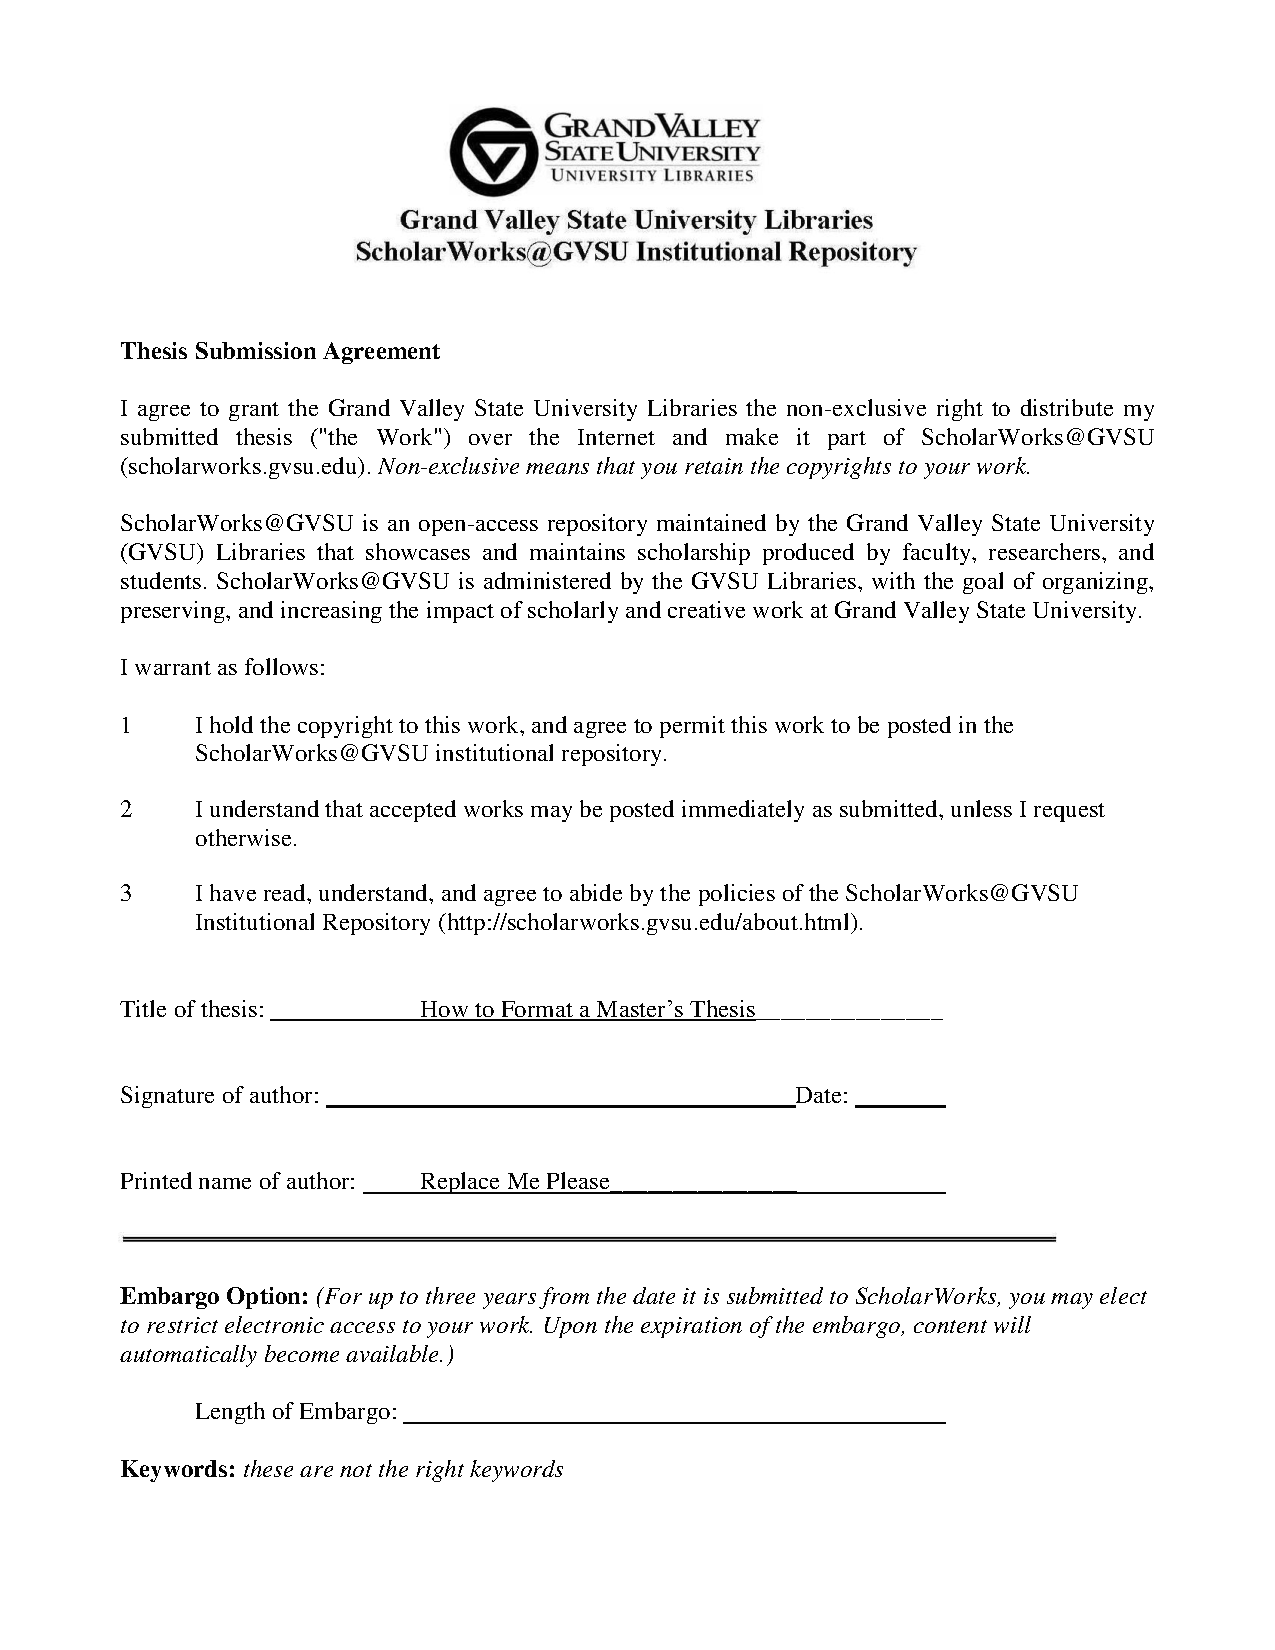
\includepdf[addtotoc={1,addsec,1,ScholarWorks Submission Agreement,scholarworks-form}]{ogs-forms/filled/scholarworks.pdf}

\end{document}

%%% Local Variables:
%%% TeX-master: "thesis"
%%% End:
